
\documentclass{article}


\usepackage[utf8]{inputenc}
\usepackage[a4paper, total={6in, 9in}]{geometry}
\usepackage{braket}
\usepackage{xcolor}
\usepackage{amsmath}
\usepackage{amsfonts}
\usepackage{tikz}
\usepackage{svg}
\usepackage{graphicx}
\usepackage{media9}
\usepackage{float}
\usetikzlibrary{calc}
\usepackage{array}
\usepackage[ruled,vlined,linesnumbered]{algorithm2e}

\usepackage[
backend=biber,
style=alphabetic,
sorting=ynt
]{biblatex}



\newcommand{\commentt}[1]{\textcolor{blue}{ \textbf{[COMMENT]} #1}}
\newcommand{\ctt}[1]{\commentt{#1}}
\newcommand{\prb}[1]{ \mathbf{Pr} \left[ {#1} \right]}
\newcommand{\onotation}[1]{\(\mathcal{O} \left( {#1}  \right) \)}
\newcommand{\ona}[1]{\onotation{#1}}
\newcommand{\nvar}[2]{ \( #1_{1}, #1_{2} ... #1_{#2}  \) }
%\newenvironment{proof}[0]{\paragraph{Proof.}}{}
%\newenvironment{remark}[0]{\textit{remark}}{}
\newenvironment{cor}[0]{\paragraph{Corollary.}}{}
\newenvironment{example}[0]{\paragraph{Example.}}{}
%\newenvironment{thm}[0]{\paragraph{Theorem.}}{}
\newtheorem{prop}{Proposition}
\newtheorem{ex}{Exercise}
\newtheorem{sol}{Solution}
\newtheorem{theorem}{Theorem} 		
\newtheorem{thm}{Theorem}[section]
\newtheorem{conj}[thm]{Conjecture} 	
\newtheorem{lemma}[thm]{Lemma}
\newtheorem{corollary}[thm]{Corollary} 
\newtheorem{claim}[thm]{Claim}
\newtheorem{proposition}[thm]{Proposition}
\newtheorem{definition}{Definition} 
\newtheorem{remark}{Remark}
 


% \addbibresource{sample.bib} %Import the bibliography file
\begin{document}    
\maketitle
\newcommand{\image}{\text{ Im } }


\begin{document}
\ifdefined\BOOK
\else
\setcounter{chapter}{8}
\fi

\chapter{Perfect Hashing and Graphs.}

In the past week, we have seen how to store keys in hash tables so that the number of mapped keys in a specific cell is $O(1)$ in expectation. The table is constructed using a hashing function $h : \text{key space} \rightarrow m \text{cells}$, randomly chosen from a universal hash function family. This function maps keys to cells, and in each cell, the keys are stored using a linked list. The cost of supported subroutines depends on the length of the list. We named any pair of different keys $x\neq y$ that are mapped to the same cell in the table, namely $h(x) = h(y)$, a collision.

Perfect hashing is a method to ensure that no collision occurs, it works only if all keys are given in advance and they are unique, meaning that the table doesn't support insertion. The idea is as follows, we sample an hash function, and then check if, for all $x,y$ in the input, it holds that $h(x)\neq h(y)$. If so then we continue. Otherwise we repeat. 

  \begin{algorithm}
  \caption{perfect-hashing($x_{1},x_{2},..x_{n}$)}
  let collision $\leftarrow$ True\\
  \While { collision } {
    collision $\leftarrow$ False\\
    let $T$ be array at length $m$ \\
    $h \leftarrow $ sample uniformly random from universal hash family $\mathcal{H}$\\
    \For { $ x \in x_{1},x_{2}..x_{n} $}{
      \If { $T_{h(x)}$ is not empty } {
       collision $\leftarrow$ True\\
       break the for-loop 
     }
     \Else{
       $T_{h(x)} \leftarrow x $ 
      }
    }
  }
  \Return $T,h$
  \end{algorithm}

  \textbf{Question.} What is the probability of choosing $h$ with no collisions on the first trial? Notice that the answer depends on $m$. (To see this, imagine the case where $m=1$. In this case, there must be collisions.) Therefore, the correct question is: for what values of $m$ do we succeed in finding a hash function with no collisions on the first trial? Let $X_{x,y}$ be the indicator of the event $h(x)=h(y)$. The expected number of collisions is then:

  \begin{equation*}
    \begin{split}
      \expp{\sum_{x\neq y}X_{x,y}} = \sum_{x\neq y}{\expp{X_{x,y}}}= { n \choose 2 } \frac{1}{m}
    \end{split}
  \end{equation*} 
Now, we would like to answer for what value of $m$ there is no collision. Therefore, if we take $m = n^{2}$, then the expected number of collisions is less than $1/2$. By the Markov inequality, the probability of having more than one collision is less than:
  \begin{equation*}
    \begin{split}
      P\left( \sum_{x\neq y}{X_{x,y}} > 1 \right) \le \expp{\sum_{x\neq y}X_{x,y}} = \frac{1}{2}
    \end{split}
  \end{equation*}
  And therefore the expected number of rounds is less than: 
  
  \begin{equation*}
    \begin{split}
      \expp{\text{ rounds }} & = \sum_{t = 0}^{\infty}t P( t \text{ rounds }) \le \sum_{t = 0}^{\infty}t \frac{1}{2^{t-1}} = O(1)
    \end{split}
  \end{equation*}  
  \textbf{Question.} What is the space complexities? We have to allocate an array at length $m$ which is $\Theta(n^{2})$ memory. Is that good? So remember that in standard hash tables, the expected number of elements that were hashed into the same cell as the key $x$ is 
  \begin{equation*}
    \begin{split}
      1 + \frac{n-1}{m} 
    \end{split}
  \end{equation*} 
   Taking $m = \Theta(n)$ is enough to ensure that the expected running time of in insertion/deletion/access is $O(1)$. This raises the question of whether the space complexity of perfect hashing can be reduced to linear.

\subsection{Perfect Hashing in Linear Space.}
%The idea is as follows, we are going to hash in two stages. The first hashing function maps keys to hash tables (instead of cells). Each hash table is constructed via the perfect hashing, and might require a space that quadric in the number of elements that stored by it (mapped in the first stage to it). So, if we denote by $n_{i}$ the number of elements that mapped into the $i$th hash table, the space cost is $\sum_{i}n_{i}^{2}$. So, now instead of starting over again when we have collision we would do it when $\sum_{i}n_{i}^{2} > 4n$. 

The idea is as follows: we will use a two-stage hashing process. In the first stage, keys will be mapped to hash tables instead of cells. Each hash table will be constructed using perfect hashing and may require a space that is quadratic in the number of elements stored in it (which were mapped to it in the first stage). Therefore, if we denote by $n_{i}$ the number of elements mapped to the $i$th hash table, the space cost will be $\sum_{i}n_{i}^{2}$. Instead of starting over when a collision occurs, we will do so when $\sum_{i}n_{i}^{2} > 4n$.
  \begin{algorithm}
  \caption{perfect-hashing-linear-space($x_{1},x_{2},..x_{n}$)}
  let toomanycollisions $\leftarrow$ True\\
  \While { toomanycollisions } {
    toomanycollisions $\leftarrow$ False\\
    let $T$ be array at length $m$ \\
    initialize any $T_{i}$ to be an empty linked list. \\ 
    $h \leftarrow $ sample uniformly random from universal hash family $\mathcal{H}$\\
    \For { $ x \in x_{1},x_{2}..x_{n} $}{
      $T_{h(x)}$.insert($x$)\\ 
      $T_{h(x)}$.size $=$ $T_{h(x)}$.size $+1$\\
    }
    \If { $\sum_{i}T_{h(i)}$.size$^{2}$ $\ge \mu$ } {
       toomanycollisions $\leftarrow$ True
     }
  }
  let $H$ be an array at length $m$\\
  \For{ $i \in [m]$}{
    $T_{i}, h_{i} \leftarrow$ hash the elements in $T_{i}$ using\\
    \ \ \ \ \ perfect hashing.
  }
  \Return $T,h$

  \end{algorithm}
  So, now it's left to show that we expect $\sum_{i} n^{2}_{i}$ to be linear, which implies that the expected number of rounds is constant.
  \begin{equation*}
    \begin{split}
      n_{i}^{2}= 2{ n_{i} \choose 2 } + n_{i}
    \end{split}
  \end{equation*}
On the other hand, $\sum_{i}{ n_{i}\choose 2  }$ is exactly the number of collisions, as for any $i$, ${ n_{i} \choose 2 }$ counts the number of distinct pairs in the $i$th table, which is equivalent to counting the number of $x\neq y$ such that $h(x) = h(y) = i$. Thus,
  \begin{equation*}
    \begin{split}
      \expp{\sum_{i}n^{2}_{i}} &= \expp{\sum_{i} {2{ n_{i} \choose 2 } + n_{i}}}= 2\cdot \expp{\text{collisions}} + \expp{\overbrace{\sum_{i}{n_i}}^{n}}\\
      &= 2 \cdot { n \choose 2} \frac{1}{m} + n
    \end{split}
  \end{equation*}
  Therefore, by choosing $m = 4n$ for the first stage, the probability of failing to choose a proper hash function is less than $1/2$.

\usetikzlibrary{positioning, arrows}
\tikzset{main node/.style={circle,draw,minimum size=0.8cm,inner sep=0pt},}
\tikzset{edge/.style = {->,> = latex'}}

\iffalse
%\newtheorem{prop}{Proposition}
%\newtheorem{ex}{Exercise}
%\newtheorem{sol}{Solution}
%\newtheorem{theorem}{Theorem} \newtheorem{thm}{Theorem}[section]
%\newtheorem{conj}[thm]{Conjecture} \newtheorem{lemma}[thm]{Lemma}
%\newtheorem{corollary}[thm]{Corollary} \newtheorem{claim}[thm]{Claim}
%\newtheorem{proposition}[thm]{Proposition}
%\newtheorem{definition}{Definition} \newtheorem{remark}{Remark}
   
%\pagestyle{empty}

%\setlength{\textwidth}{6.5in}
%\setlength{\evensidemargin}{0.0in}
%\setlength{\oddsidemargin}{0.0in}
%\setlength{\topmargin}{-0.25in}
%\setlength{\textheight}{9.0in}
%\setlength{\baselineskip}{1.3\baselineskip}
%\setlength{\parindent}{.0in}
\fi
\tikzset{
node of list/.style = { 
             draw, 
             fill=orange!20, 
             minimum height=6mm, 
             minimum width=6mm,
             node distance=6mm
   },
link/.style = {
     -stealth,
     shorten >=1pt
     },
array element/.style = {
    draw, fill=white,
    minimum width = 6mm,
    minimum height = 10mm
  }
}

\def\LinkedList#1{%
  \foreach \element in \list {
     \node[node of list, right = of aux, name=ele] {\element};
     \draw[link] (aux) -- (ele);
     \coordinate (aux) at (ele.east);
  } 
}



%%%%%%%%%%%%%%%%%%%%%%%%%%%%%%%%%%%%%%%%%%%%%%%%%%%%%%%%%%%%



%%%%%%%%%%%%%%%%%%%%%%%%%%%%%%%%%%%%%%%%%%%%%%%%%%%%%%%%%%%%

%\vspace{0.2in}

\section{Graphs}
%This is an important section, as you'll see graphs A LOT in this course and in the courses to follow. 

\subsection{Definitions, Examples, and Basics}

\begin{figure}[h]
\begin{subfigure}[b]{0.65\textwidth}
\begin{definition}
A \textbf{non-directed graph} $G$ is a pair of two sets - $G=(V, E)$ - $V$ being a set of vertices and $E$ being a set of couples of vertices, which represent edges ("links") between vertices.
\end{definition}

\textbf{Example}: $G= (\{1,2,3,4\},\ \{\{1,2\}, \{1,3\}, \{3,4\}\})$ is the following graph:\\ 
\end{subfigure}
\begin{subfigure}[b]{0.05\textwidth}
  \
\end{subfigure}
  \begin{subfigure}[b]{0.25\textwidth}
    \begin{tikzpicture}
\node[main node](1){$1$};
\node[main node](2)[below = 1cm of 1]{$2$};
\node[main node](3)[right = 1cm of 1]{$3$};
\node[main node](4)[below = 1cm of 3]{$4$};

\path[draw, thick]
(1) edge node {} (2)
(1) edge node {} (3)
(3) edge node {} (4);
\end{tikzpicture}
\end{subfigure}
\end{figure}
\begin{figure}[h]
\begin{subfigure}[b]{0.65\textwidth}
\begin{definition}
A \textbf{directed graph} $G$ is a pair of two sets - $G=(V, E)$ - $V$ being a set of vertices and $E\subseteq V\times V$ being a set of directed edges ("arrows") between vertices.
\end{definition}
\textbf{Example}: $G=(\{1,2,3,4\},\ \{(1, 2), (1, 4), (4, 1), (4,3)\})$ is the following graph (note that it has arrows): \\ 
\end{subfigure}
\begin{subfigure}[b]{0.05\textwidth}
  \
\end{subfigure}
  \begin{subfigure}[b]{0.25\textwidth}
    \begin{tikzpicture}
\node[main node](1){$1$};
\node[main node](2)[below = 1cm of 1]{$2$};
\node[main node](3)[right = 1cm of 1]{$3$};
\node[main node](4)[below = 1cm of 3]{$4$};

\draw[edge] (1) to (2);
\draw[edge] (1) to (4);
\draw[edge] (4) to (1);
\draw[edge] (4) to (3);
\end{tikzpicture}
\end{subfigure}
\end{figure}

\begin{definition}
  A \textbf{weighted graph} composed by a graph $G=\left( V,E \right)$ (either non-directed or directed) and a weight function $w : E \rightarrow \mathbb{R}$. Usually (but not necessary), we will think about the quantity $w(e)$, where $e \in E$, as the length of the edge.  
\end{definition}

Now that we see graphs with our eyes, we can imagine all sorts of uses for them... For example, they can represent the structure of the connections between friends on Facebook, or they can even represent which rooms in your house have doors between them.

\begin{remark}
Note that directed graphs are a \textbf{generalization} of non-directed graphs, in the sense that every non-directed graph can be represented as a directed graph. Simply take every non-directed edge $\{v,u\}$ and turn it into two directed edges $(v,u), (u,v)$. 
\end{remark}

\begin{remark}
Note that most of the data structures we discussed so far - Stack, Queue, Heap, BST - can all be implemented using graphs.
\end{remark}

Now let's define some things in graphs:

\begin{definition} (Path, circle, degree)
\begin{enumerate} 
\item A \textbf{simple path} in the graph $G$ is a series of unique vertices (that is, no vertex appears twice in the series) $v_1, v_2, ..., v_n$ that are connected with edges in that order. 
\item A \textbf{simple circle} in the graph $G$ is a simple path such that $v_1 = v_n$. 
\item The \textbf{distance} between two vertices $v,u\in V$ is the length of the shortest path between them ($\infty$ if there is no such path).
\end{enumerate}
\end{definition}

\begin{remark}
Note that for all $u,v,w\in V$ the triangle inequality holds regarding path lengths. That is:
$$dist(u,w)\leq dist(u,v) + dist(v, w)$$
\end{remark}

\begin{definition} (connectivity)
\begin{enumerate}
  \item Let $ G =\left( V,E \right)$ be a non-directed graph. A \textbf{connected component} of $G$ is a subset $U \subseteq V$ of maximal size in which there exists a path between every two vertices. 
\item A non-directed graph $G$ is said to be a \textbf{connected} graph if it only has one connected component.
\item Let $ G = \left(V, E\right)$ be a directed graph. A \textbf{strongly connected component} of $G$ is a subset $U \subseteq V$ of maximal size in which for any pair of vertices $u,v \in U$ there exist both directed path from $u$ to $v$ and a directed path form $v$ to $u$.   
\end{enumerate}
\end{definition}
%\begin{figure}[h]
  %\begin{subfigure}[b]{0.4\textwidth} 
%An \textbf{example} of a non-connected graph: \\ \\ \\  \\
%\end{subfigure}
%\begin{subfigure}[b]{0.05\textwidth}
  %\
%\end{subfigure}
%\begin{subfigure}[b]{0.25\textwidth}
%\begin{tikzpicture}
%\node[main node](1){$1$};
%\node[main node](2)[below = 1cm of 1]{$2$};
%\node[main node](3)[right = 1cm of 1]{$3$};
%\node[main node](4)[below = 1cm of 3]{$4$};
%
%\draw[edge] (1) to (2);
%\draw[edge] (3) to (4);
%\end{tikzpicture}
%\end{subfigure}
%\end{figure}

\begin{claim}
Let $G=(V,E)$ be some graph. If $G$ is connected, then $|E| \geq |V|-1$
\end{claim}

\begin{proof}
We will perform the following process: Let $\{e_1,...,e_m\}$ be an enumeration of $E$, and let $G_0=(V,\emptyset)$. We will build the graphs $G_1, G_2,... G_m=G$ by adding edges one by one. Formally, we define - 
$$\forall i\in[m]\ \ G_i=(V,\{e_1,...,e_i\})$$
$G_0$ has exactly $|V|$ connected components, as it has no edges at all. Then $G_1$ has $|V|-1$. From there on, any edges do one of the following:
\begin{enumerate}
    \item Keeps the number of connected components the same (the edge closes a cycle)
    '\item Lowers the number of connected components by $1$ (the edges does not close a cycle)
\end{enumerate}

So in general, the number of connected components of $G_i$ is $\geq |V|-i$. 
Now, if $G_m=G$ is connected, it has just one connected component! This means:
$$1 \geq |V| - |E|\ \implies \ |E|\geq|V|-1$$

\end{proof}


\subsection{Graph Representation}

Okay, so now we know what graphs are. But how can we represent them in a computer? There are two main options. The first one is by \textbf{array of adjacency lists}. Given some graph $G$, every slot in the array will contain a linked list. Each linked list will represent a list of some node's neighbors. The second option is to store edges in an \textbf{adjacency matrix}, a $ |V| \times |V| $ binary matrix in which the $v,u$-cell equals $1$ if there is an edge connecting $u$ to $v$. That matrix is denoted by $A_{G}$ in the example below. Note that the running time analysis might depend on the underline representation.     

\textbf{Question.} What is the memory cost of each of the representations? Note that while holding an adjacency matrix requires storing $|V|^2$ bits regardless of the size of $E$, Maintaining the edges by adjacency lists costs linear memory at the number of edges and, therefore, only $ \Theta \left(  |V| + |E| \right) $ bits. 

\paragraph{Example.} Consider the following directed graph:
\begin{figure}[h]
  \centering
  \begin{subfigure}[b]{0.25\textwidth}
    \begin{tikzpicture}
      \node[main node](1){$1$};
      \node[main node](2)[below = 1cm of 1]{$2$};
      \node[main node](3)[right = 1cm of 1]{$3$};
      \node[main node](4)[below = 1cm of 3]{$4$};

      \draw[edge] (1) to (2);
      \draw[edge] (1) to (4);
      \draw[edge] (4) to (1);
      \draw[edge] (4) to (3);
      \draw[edge] (1) to (3);
      \draw[edge] (3) to (1);
    \end{tikzpicture}  
    \\ \\  
  \end{subfigure} 
  \begin{subfigure}[b]{0.49\textwidth}
    \begin{tikzpicture}
      \foreach \index/\list in {1/{2,3,4,null}, 2/{null}, 3/{1, null}, 4/{1, 3, null}} {
	\node[array element] (aux) at (0,-\index) {\index};
	\LinkedList{\list}
      }
    \end{tikzpicture}  
  \end{subfigure}
  \caption{ Persenting $G$ by array of adjacency lists.  }
\end{figure}

%Its representation will be: \\ \\

\begin{figure}[h]
  \centering
  \begin{subfigure}[b]{0.25\textwidth}
        \begin{tikzpicture}
\node[main node](1){$1$};
\node[main node](2)[below = 1cm of 1]{$2$};
\node[main node](3)[right = 1cm of 1]{$3$};
\node[main node](4)[below = 1cm of 3]{$4$};

\draw[edge] (1) to (2);
\draw[edge] (1) to (4);
\draw[edge] (4) to (1);
\draw[edge] (4) to (3);
\draw[edge] (1) to (3);
\draw[edge] (3) to (1);
\end{tikzpicture} \\ 
  \end{subfigure}
\begin{subfigure}[b]{0.49\textwidth}       
  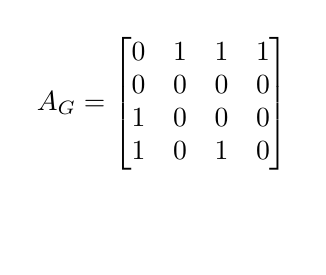
\begin{tikzpicture}
    \node (1) at (0,0) { };
    \node  (2) at (1,1.7) { $ A_{G} = 
	  \begin{bmatrix}
	0 & 1 & 1 & 1\\
	0 & 0 & 0 & 0\\
	1 & 0 & 0 & 0\\
	1 & 0 & 1 & 0
	\end{bmatrix}
      $ };
      \end{tikzpicture}
\end{subfigure}
\caption{ Presenting $G$ by adjacency matrix. }
\end{figure}

\subsection{Breadth First Search (BFS)}

One natural thing we might want to do is to travel around inside a graph. That is, we would like to visit all of the vertices in a graph in some order that relates to the edges. 
Breadth-first search constructs a breadth-first tree, initially containing only its root, which is the source vertex $s$. Whenever the search discovers a white vertex $v$ in the course of scanning the adjacency list of a gray vertex $u$, the vertex $v$ and the edge ($u$, $v$) are added to the tree. We say that $u$ is the predecessor or parent of $v$ in the breadth-first tree. Since every vertex reachable from $s$ is discovered at most once, each vertex reachable from $s$ has exactly one parent. (There is one exception: because $s$ is the root of the breadth-first tree, it has no parent.) Ancestor and descendant relationships in the breadth-first tree are defined relative to the root $s$ as usual: if $u$ is on the simple path in the tree from the root $s$ to vertex $v$, then $u$ is an ancestor of $v$, and $v$ is a descendant of $u$.

The breadth-first-search procedure BFS on the following page assumes that the graph $G = (V, E)$ is represented using adjacency lists. It denotes the queue by $Q$, and it attaches three additional attributes to each vertex $v$ in the graph:

\begin{enumerate}
    \item $v$.visited is a boolean flag which indicate wheter $v$ was allready visited.
    \item $\pi(v)$ is $v$’s predecessor in the breadth-first tree. If $v$ has no predecessor because it is the source vertex or is undiscovered, then $\pi(v)$ is None/NULL.
\end{enumerate}

  \begin{algorithm}
  \caption{BFS($G, s$)}
    \For {$v\in V$}{
	 $v.visited \leftarrow $ False 
     }
 $Q\leftarrow$ new Queue \\ 
 $Q$.Enqueue($s$) \\
 $s$.visited $\leftarrow$ True \\
 \While {$Q$ is not empty} {
 $u\leftarrow Q$.Dequeue() \\
	\For {neighbor $w$ of $u$} {
	\If {$w$.visited is False}{
		 $w$.visited$\leftarrow$ True \\
		 $\pi(w) \leftarrow u $ \\
		 $Q$.Enqueue($w$)

	      }
	}
      }
  \end{algorithm}

\underline{Correctness}: The example should be enough to explain the correctness. A concrete proof can be found in the book, page 597.

\underline{Runtime}: We can analyse the runtime line-by-line:
\begin{itemize}
\item Lines 1-2: $|V|$ operations, all in $O(1)$ runtime, for a total of $O(|V|)$.
\item Lines 3-6: $O(1)$
\item Lines 7-8: First we need to understand the number of times the $while$ loop iterates. We can see that every vertex can only enter the queue ONCE (since it is then tagged as "visited"), and therefore it runs $\leq |V|$ times. All operations are $O(1)$, and we get a total of $O(|V|)$. 
\item Lines 9-13: Next, we want to understand the number of times this $for$ loop iterates. 
The for loop starts iterating once per vertex, and then the number of its iterations is the same as the number of neighbors that this vertex has. Thus, it runs $O(|E|)$ times.
\end{itemize}
So all in all we get a runtime of $O(|V|+|E|)$


\subsection{Paths in the BFS Tree are Shortest Paths.}
We are about to prove a useful property of BFS scanning: the algorithm discovers vertices in the order of their distance from the source. In particular, $\pi$ defines a tree in which the path from $s$ to $u$ is the shortest path in the original graph $G$ from $s$ to $u$.

  \begin{claim}
    Consider the $\pi$ returned from running the BFS routine on vertex $s$. Let $\delta(u)$ denote the distance between $u$ and $s$. Then,
\begin{enumerate}
    \item For every $u$ and $w$ where $\delta(u) < \delta(w)$, $u$ will be extracted from the queue before $w$.
    \item $\delta(u) = \delta(\pi(u)) + 1$. 
  \end{enumerate}
  \end{claim}
  \begin{proof}
    By induction, on $\delta(u)$.
    \begin{enumerate}
      \item  Base. Consider $u$ and $w$ such that $\delta(u) = 0$ and $\delta(w) > 0$. In this case, $u$ is $s$, and the statement holds by definition. Furthermore, for any vertex $u$ that is a neighbor of $s$, the algorithm sets $\pi(u) \leftarrow v$, and it is easy to see that $\delta(u) = 1 = 1 + \delta(v)$.
      \item Assumption. Assuming correctness for any $u$ such that $\delta(u) < m$ and $\delta(w) > \delta(u)$, $u$ is extracted before $w$. Additionally, for any $u$ such that $\delta(u) \le m$, it holds that $\delta(u) = \delta(\pi(u)) + 1$.
      \item Step. Consider a vertex $u$ such that $\delta(u) = m$, and let $w$ be a vertex such that $\delta(w) > \delta(u)$. If $w$ does not enter the queue at all, then the statement holds trivially. Suppose it does, so $\pi(w)$ is defined.

        Let $y$ be $\pi(w)$, and we can assume that $\delta(y) = m$, otherwise we repeat the proof by taking $y$ instead of $w$ as the vertex at distance $\delta(y) > \delta(u)$. This is because, by definition, $\pi(w)$ is extracted before $w$, Thus proving that $\pi(w)$ extracted after $u$ is sufficient. 

        Let $y^{\prime}$ be the vertex such that $\pi(u) = y^{\prime}$. By the second property, we have $\delta(y^\prime) = m - 1$. Therefore, using the induction assumption again, $y^{\prime}$ is extracted before $y$. This means that $y^\prime$ enqueues $u$ before $y$ is extracted from the queue, and will be extracted before any of the successors (according to $\pi$) of $y$ are extracted, including $w$. 

        
        It remains to be shown that any vertex $u$ such that $\delta(u) = m+1$ satisfies $\delta(u) = \delta(\pi(u)) + 1$. Suppose not, which means that either $\delta(\pi(u))$ also does not satisfy the equality, contradicting the induction assumption, or that $\delta(\pi(u)) > m$. Let $\braket{s,v_1 ,v_2, .. ,v_{m},u}$ be the minimal path between $s$ and $u$, where $\delta(v_m) = m$. As shown earlier, $v_m$ is removed from the queue before $\pi(u)$, and at the time of its removal, $u$ is not yet colored. Therefore, by the definition of the algorithm, $\pi(u)$ is set to be $v_m$, which contradicts the assumption that $\delta(\pi(u)) > m$.
    \end{enumerate}
  \end{proof}

\subsection{Usage of BFS}
Now we have a way to travel through a graph using the edges. How else can we use it?\\ \\ 
\textbf{Exercise}: Present and analyse an algorithm $CC(G)$ which receives some undirected graph $G$ and outputs the number of connected components in $G$ in $O(|V|+|E|)$. \\

\textbf{Solution}: Consider the following algorithm: 

  \begin{algorithm}
  \caption{CC($G$)}
     count $\leftarrow 0$\\
     \For {$v\in V$ }{
	\If {$v$.visited = False} {
	  count$\leftarrow$count$+1$ \\
	  BFS($G, v$)
	}
      }
	\Return count
  \end{algorithm}

  \ifdefined\DFS
%Consider a vertex $u$ such that $\delta(u) = m$, and let $w$ a vertex such $\delta(w) > \delta(u)$. If $w$ doesn't enter at all into the queue then the state holds trivially. Suppose it is, so $\pi(w)$ is defined. Let $y$ be the vertex such $y = \pi(\pi(\pi(..\pi(w))))$ and also $\delta(y)= m$. And let $y^{\prime}$ be the vertex such $\pi(u) = y^{\prime}$. By the second property we have that $\delta(y^\prime) = m - 1$ therefore using again the induction assumption, $y^{\prime}$ is extracted before $y$. Therefore $y^\prime$ enqueues $u$ before $y$ is extracted form the queue, and will be extracted before any of the successors (according to $\pi$) of $y$ will be extracted including $w$. 
        
        %Consider a vertex $u$ such that $\delta(u) = m$, and let $w$ be a vertex such that $\delta(w) > \delta(u)$. If $w$ does not enter the queue at all, then the statement holds trivially. Suppose it does, so $\pi(w)$ is defined. Let $y$ be $\pi(w)$, we can assume that $\delta(y) = m$, otherwise we repeat on the proof but taking $y$ instead $w$ as the vertex at distance $\delta(y) > \delta(u)$, as by definition $\pi(w)$ is extracted before $w$ proving that $\pi(w)$ extracted after $u$ is sufficient. And let $y^{\prime}$ be the vertex such that $\pi(u) = y^{\prime}$. By the second property, we have that $\delta(y^\prime) = m - 1$. Therefore, using the induction assumption again, $y^{\prime}$ is extracted before $y$. This means that $y^\prime$ enqueues $u$ before $y$ is extracted from the queue, and will be extracted before any of the successors (according to $\pi$) of $y$ are extracted, including $w$.

\subsection{Depth First Search (DFS)}
As its name implies, depth-first search searches "deeper" in the graph whenever possible. Depth-first search explores edges out of the most recently discovered vertex $v$ that still has unexplored edges leaving it. Once all of $ v$'s edges have been explored, the search "backtracks" to explore edges leaving the vertex from which $v$ was discovered. This process continues until all vertices that are reachable from the original source vertex have been discovered. If any undiscovered vertices remain, then depth-first search selects one of them as a new source, repeating the search from that source. The algorithm repeats this entire process until it has discovered every vertex.

  \begin{algorithm}
  \caption{DFS($G$)}
   \bf{DFS}( $G$): \\
    \For {$v\in V$}{
 	$vi$.visited $\leftarrow False$
    }
    time $ \leftarrow 1 $\\
    \For {$v\in V$}{
      \If { not $v$.visited } {
	$\pi \left( v \right)  \leftarrow $ null \\ 
	Explore( $G,v$ ) 
     } 
   }

  \end{algorithm}

  \begin{algorithm}[H]
    \bf{Explore}($G,v$): \\
     Previsit($v$)
    \For {$\left( v,u \right) \in E  $}{
      \If { not $u$.visited } {
	$ \pi \left( u \right) \leftarrow v $ \\ 
	Explore( $G, u$ ) 
      }
    }
    Postvisit($v$)
  \end{algorithm}
  \begin{algorithm}[H]
    \bf{Previsit}($v$): \\
    pre($v$) $\leftarrow $ time \\
    time $\leftarrow$ time $+1$
  \end{algorithm}
  \begin{algorithm}[H]
   \bf{Postvisit} ($v$): \\ 
    post($v$) $\leftarrow $ time \\
    time $\leftarrow$ time $+1$
  \end{algorithm}


\paragraph{Properties of depth-first search.} Depth-first search yields valuable information about the structure of a graph. Perhaps the most basic property of depth-first search is that the predecessor subgraph $G_{\pi}$ does indeed form a forest of trees since the structure of the depth-first trees exactly mirrors the structure of recursive calls of explore-function. That is, $u$ = $\pi\left( v \right)$ if and only if explore($G, v$) was called during a search of $ u$'s adjacency list. Additionally, vertex $v$ is a descendant of vertex $u$ in the depth-first forest if and only if $v$ is discovered during the time in which $u$ is gray.
Another important property of depth-first search is that discovery and finish times have a parenthesis structure. If the explore procedure were to print a left parenthesis "$(u$" when it discovers vertex $u$ and to print a right parenthesis r``$u)$" when it finishes $u$, then the printed expression would be well-formed in the sense that the parentheses are properly nested.

The following theorem provides another way to characterize the parenthesis structure.

\begin{claim}[Parenthesis theorem]
In any depth-first search of a (directed or undirected) graph $G = (V, E)$, for any two vertices $u$ and $v$, exactly one of the following three conditions holds:

\begin{enumerate}
  \item the intervals [pre($u$), post($u$)] and [pre($v$), post($v$)] are entirely disjoint, and neither $u$ nor $v$ is a descendant of the other in the depth-first forest.
  \item the interval [pre($u$), post($u$)] is contained entirely within the interval [pre($v$), post($v$)], and $u$ is a descendant of $v$ in a depth-first tree, or
  \item the interval [pre($v$), post($v$)] is contained entirely within the interval [pre($u$), post($u$)], and $v$ is a descendant of $u$ in a depth-first tree.
  \end{enumerate}
\end{claim}

\begin{proof} We begin with the case in which pre($u$) $<$ pre($v$). We consider two subcases, according to whether pre($v$) $<$ post($u$). The first subcase occurs when pre($v$) $<$ post($u$), so that $v$ was discovered while $u$ was still gray, which implies that $v$ is a descendant of $u$. Moreover, since $v$ was discovered after $u$, all of its outgoing edges are explored, and $v$ is finished before the search returns to and finishes $u$. In this case, therefore, the interval [pre($v$), post($v$)] is entirely contained within the interval [pre($u$), post($u$)]. In the other subcase, post($u$) $<$ pre($v$), and by defintion, pre($u$) $<$ post($u$) $<$ pre(v) $<$ post($v$), and thus the intervals [pre($u$), post($u$)] and [pre($v$), post($v$)] are disjoint. Because the intervals are disjoint, neither vertex was discovered while the other was gray, and so neither vertex is a descendant of the other.
\end{proof}


\paragraph{  Corollary. Nesting of descendants' intervals.}
  Vertex $v$ is a proper descendant of vertex $u$ in the depth-first forest for a (directed or undirected) graph $G$ if and only if pre($u$) $<$ pre($v$) $<$ post($v$) $<$ post($u$).
\fi


% \printbibliography 
\end{document}


